\chapter{Supply and Demand}
Concepts of supply and demand form the very foundations of economics. The interactions between supply and demand decide the price of a product. It is best to explain them by using an example. Let us take an agricultural produce, brinjal (good of interest) and see how restaurants (bulk consumers) would react to different price points (offering prices) and how farmers (producers) would react to different price points (asking prices).  A transaction (a purchase) happens when the asking price and the offering price are the same (so both are satisfied).

\section{Nature of Demand}
Restaurants have limited weekly budgets for vegetables. Based on the prices of different vegetables, they will have to decide how much of brinjal to buy, how much of potatoes to buy, how much of capsicum to buy and so on. 

\marginnote{Demanded quantity falls when offering prices of that good increases}Coming to our good of interest, if the offering price of brinjal is Rs. 30/kg, then, let us say restaurants in Pune overall will buy 200 tonnes of brinjal. But, if the price of brinjal were to go up, to say Rs, 70/kg, it is intuitive that restaurants would buy lesser quantity of brinjal and instead would buy more of some other vegetable. If the price of brinjal goes even higher, the restaurants would buy even lesser brinjal. 

On the other hand, if price of brinjal were to go to a lower value, say, Rs. 40/kg, it is conceivable that restaurants would now increase the consumption of brinjal at the expense of a more pricy vegetable. And if the price of brinjal falls even further, consumption of it will increase even further.

To conclude, demand falls as price rises and vice versa. This is depicted in \autoref{fig:demandCurve}.
	\begin{figure}[h]
		\centering
		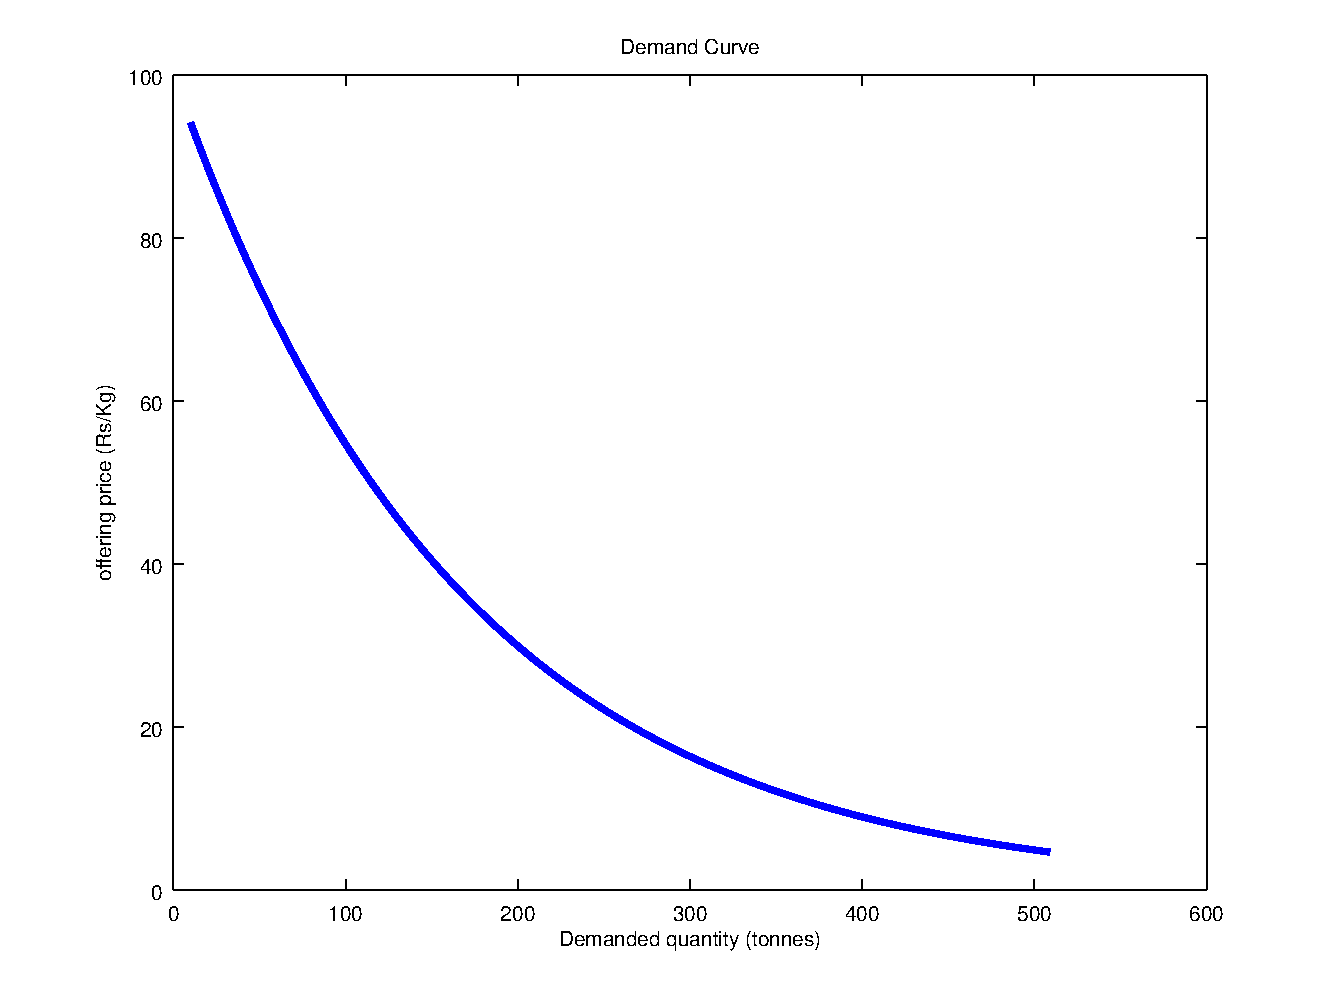
\includegraphics[width = \textwidth]{supplyDemand/demandCurve}
		\caption{The Demand Curve}
		\label{fig:demandCurve}
	\end{figure}
	
\section{Nature of Supply}
\marginnote{Supplied quantity falls when asking prices of that good decreases}The nature of supply is exactly opposite to that of the demand. As the asking price of the good increases, supply also increases. The higher the asking price of brinjal, the more incentive there is for the farmers to grow brinjal instead of some other vegetable. So as the asking price of brinjal increases, more and more farmers will grow brinjal and hence there will be more and more supply of brinjal in the market. A hypothetical supply curve for brinjal may look like \autoref{fig:supplyCurve}.

	\begin{figure}[h]
		\centering
		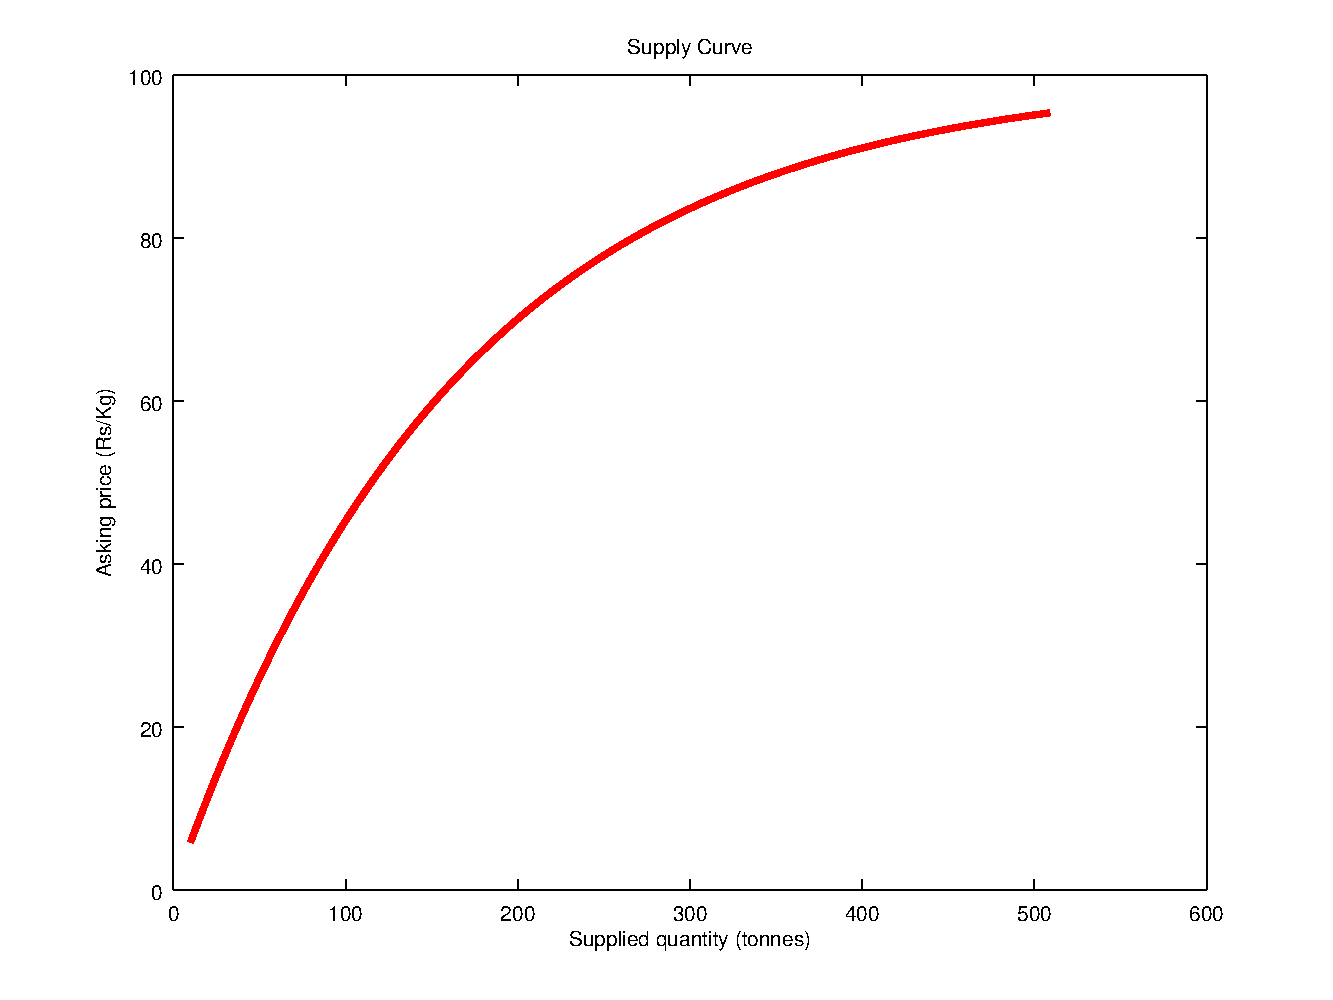
\includegraphics[width = \textwidth]{supplyDemand/supplyCurve}
		\caption{The Supply Curve}
		\label{fig:supplyCurve}
	\end{figure}
	
\section{Transaction}
\marginnote{Transaction happens when supplier and consumer like the price point for a certain qty of goods}Remember that, the quantities we have so far talked about, namely, offering price, asking price, supplied quantity, demanded quantity, are just hypothetical values - In other words, the demanded quantity \emph{would be} 200 tonnes, \emph{if} the offering price is Rs. 30/kg. This doesn't mean brinjal would ever be offered at Rs. 30/kg or that 200 tonnes of brinjal will be transacted. Similarly, on the supply side, again we hypothesize that, \emph{if} the asking price is Rs. 70/kg, then 200 tonnes of brnijal \emph{would be} supplied. That doesn't mean consumers would ever be willing to pay Rs. 70/kg and 200 tonnes of brinjal will be transacted. Thus the supply and demand curve need to be thought of as a result of a ``what if'' survey answered by producers and customers  and not as the result of some real life transactions.

A transaction can happen only when supplier agrees to supply a certain quantity of brinjal at a price that the consumer is willing to pay for that quantity of brinjal. Mathematically speaking, this happens where the supply curve meets the demand curve. And that point would eventually decide how many tonnes of brinjal was actually transacted and at what price. 

	\begin{figure}[h]
		\centering
		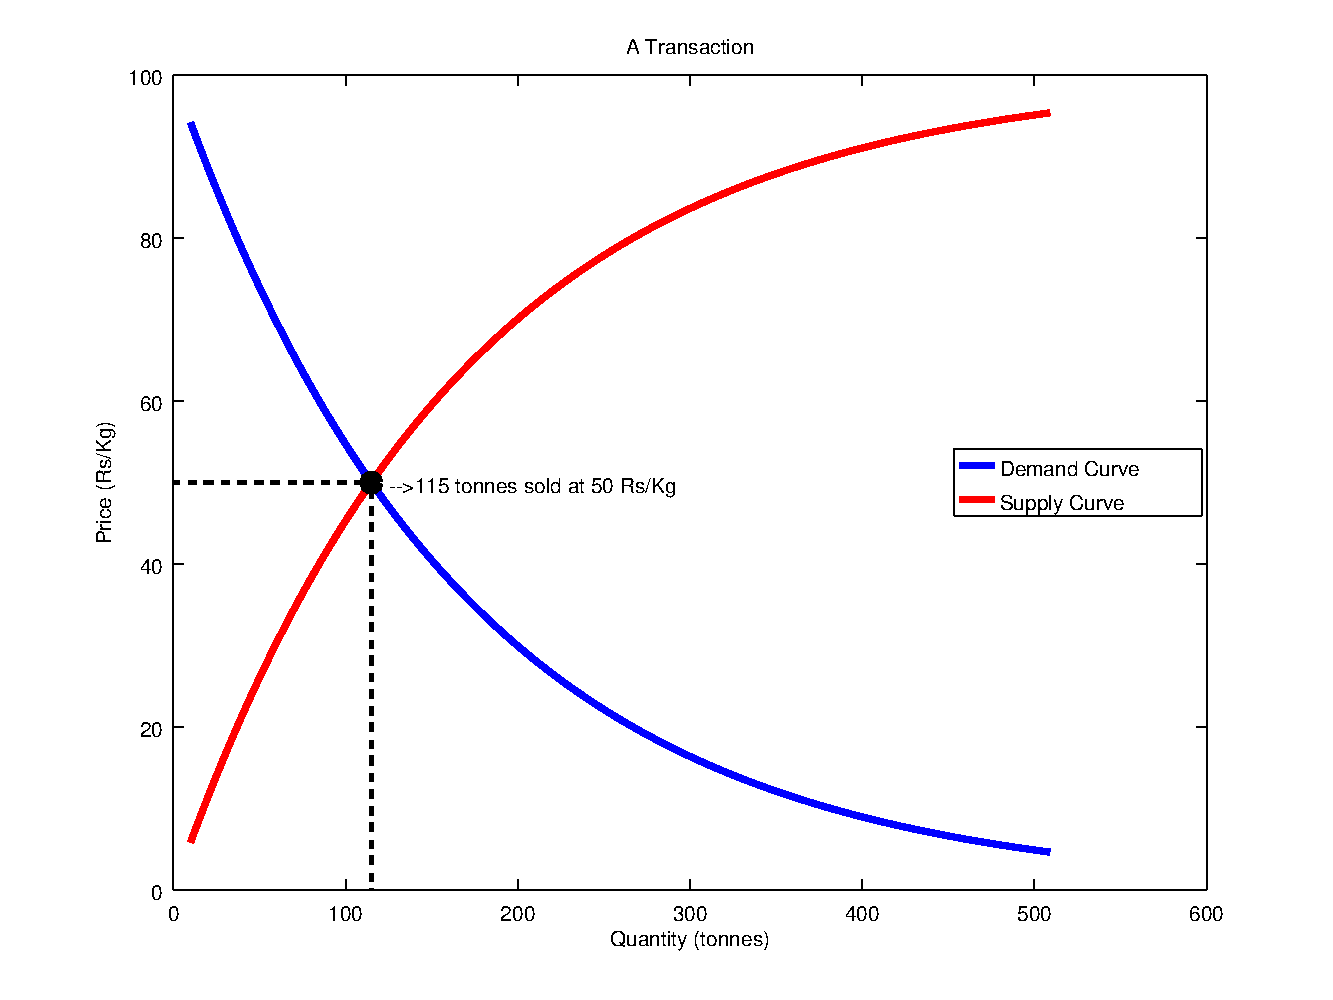
\includegraphics[width = \textwidth]{supplyDemand/transaction}
		\caption{A Transaction}
		\label{fig:transactionPoint}
	\end{figure}
	
As you can see from \autoref{fig:transactionPoint}, in our case a transaction happened at a price point for a given quantity that was acceptable to both the parties. This transaction point is where the ``what if'' hypothetical scenarios end and a real deal happens. You can see that now the x and y axes are denoted as ``quantity'' and ``price'' as opposed to hypothetical terms like ``demanded quantity'' or ``Offering price''. 

It is important to note that, though hypothetically, consumers may want to buy more brinjal than the actual trasacted quantity of 115 tonnes, they just didn't have a choice as supplier wasn't willing to supply more than 115 tonnes and consumer wasn't willing to pay more than 50 Rs/kg. 

\section{Caveats}
The supply and demand theory described in prior sections give us a good framework to understand economics at a very basic level. However it hides a lot of nuances as discussed in the following subsections.

\subsection{Simple Supply Demand Curves are Macroeconomic Model}
The simple supply demand curves we dealt above describe us the situation in an average sense. In reality, though we said that 115 tonnes of brinjal was transacted at Rs. 50/kg, it is not that every single transaction happened at Rs. 50/kg. It is possible that 75 tonnes were transacted at 42 Rs/kg and 40 tonnes were transacted at 65 Rs/kg. So our demonstrated transaction point of 50 Rs/kg is merely so in an average sense, i.e., (75*42 + 40*65)/(75+40) = 50.

There are several reasons why two transactions happened at two different prices:
\begin{itemize}
	\item Some party may not have market intelligence to know what other parties are generally offering/asking the commodity at
	\begin{itemize}
		\item How often do people have access about supply-demand data? Even if they had, how often is the data usable in decision making? - The data could be too old or irrelevant to the local context
	\end{itemize}
	\item Human factor is involved: Some are good at bargaining, some aren't. Some customers may have strong preferences for certain suppliers based on trust built over years
\end{itemize}	

\subsection{Not Everyone is a Rational Actor}
How many of us approach the act of selling/purchasing some brinjal methodically considering market intelligence (even when it is available), the price of alternatives (other vegetables) etc.? Big restaurant chains may make choices methodically, but small restaurant owners may buy things based on imperfect and rough calculations.

\subsection{Many Supply and Demand Curves}
Even though we have shown a single supply and single demand curve, they are so just in an average sense and do not reflect the price preferences of every individual involved in brijal transactions. For instance, in expensive restaurants the cost of raw materials (vegetables) could only constitute a very small fraction of the price of the dishes and may not bother to switch the supplier just because s/he is quoting a slightly higher price for brinjal than the rest of the market. Another example could be that there is a restaurant that is famous just for their baingan barta - unlike others, this customer won't switch to an alternative vegetable as the offering price changes.

\section{Lateral Shifts in Supply/Demand Curves}
There are many factors that affect the supply and demand curves. Some of them cause the curves to retain their shapes, but shift laterally - to the right of the left. For instance, if the purchasing capacity of the entire population went up due to strong development in the country, the demand curve could shift right. If fuel prices increase, the supply curve could shift left. This is demonstrated pictorially in Figures \autoref{fig:demandRightCurve}, \autoref{fig:supplyLeftCurve}.

	\begin{figure}[h]
		\centering
		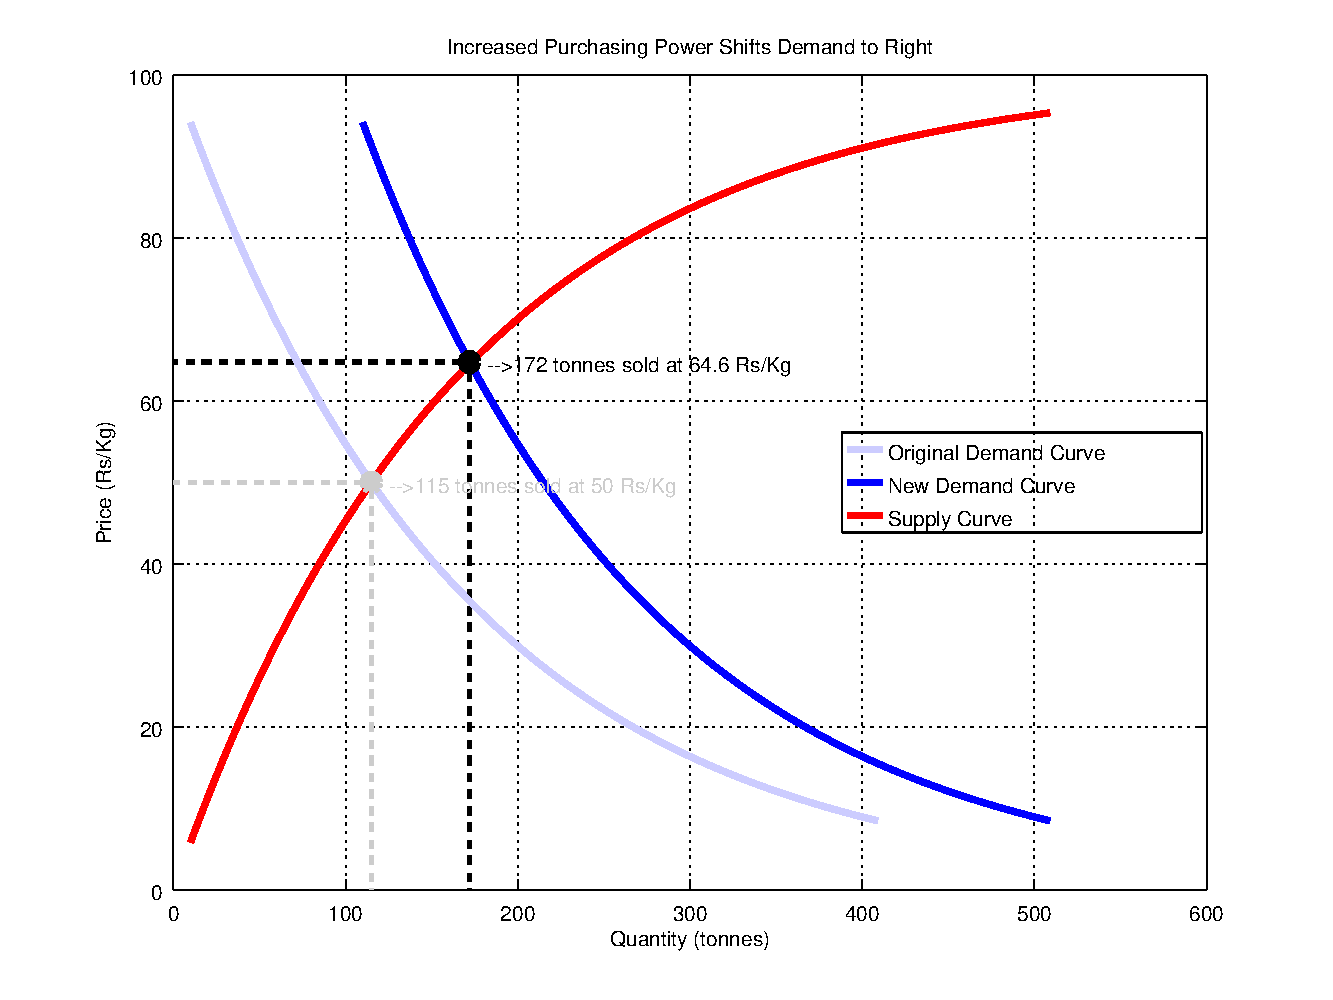
\includegraphics[width = \textwidth]{supplyDemand/rightShiftDemand}
		\caption{Demand Shifts Right}
		\label{fig:demandRightCurve}
	\end{figure}
	
	\begin{figure}[h]
		\centering
		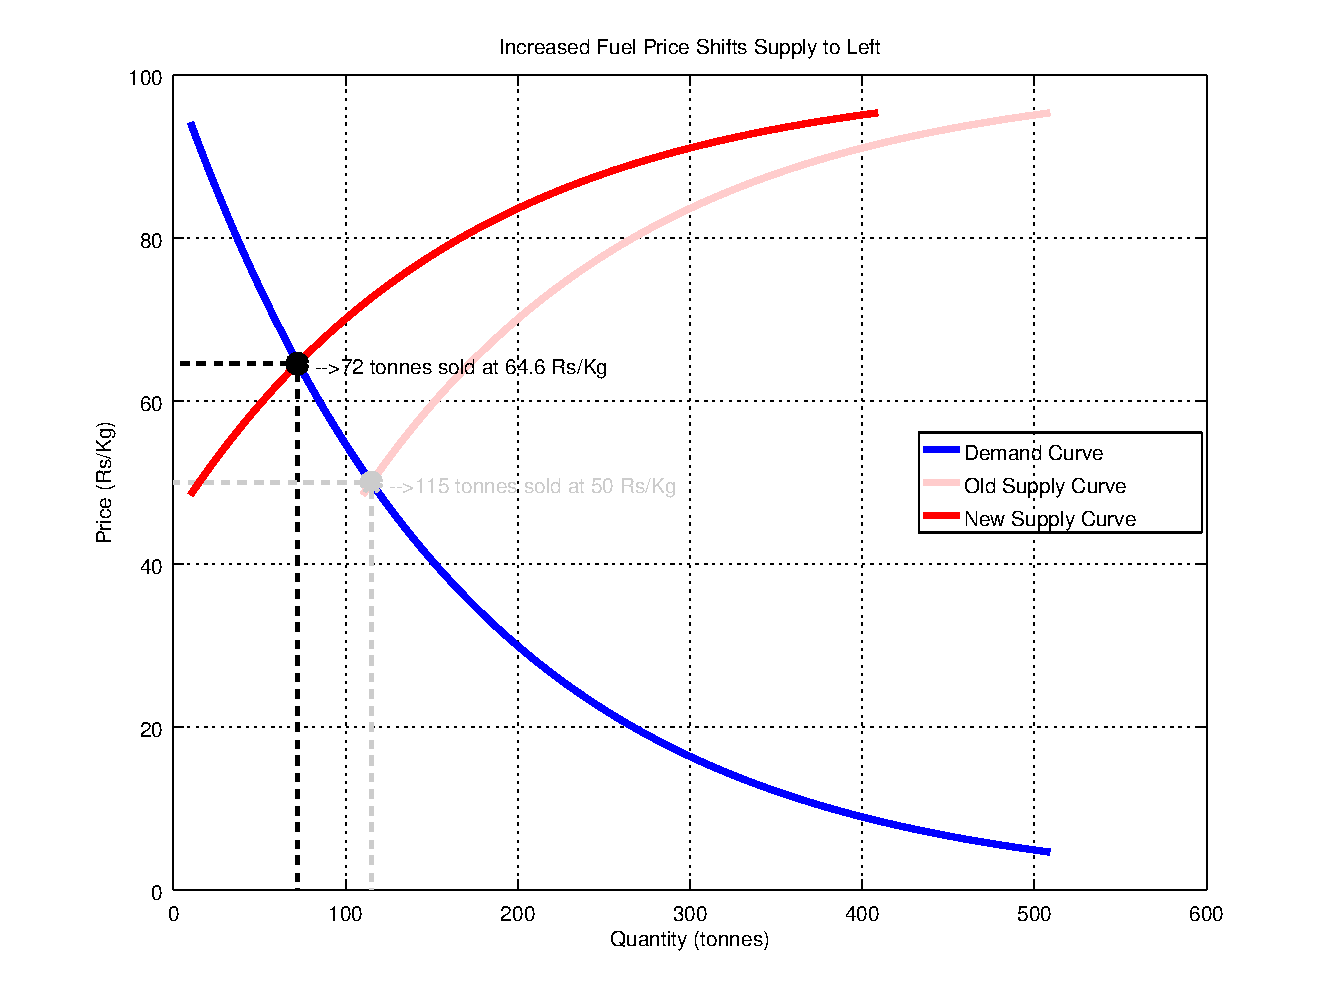
\includegraphics[width = \textwidth]{supplyDemand/leftShiftSupply}
		\caption{Supply Shifts Left}
		\label{fig:supplyLeftCurve}
	\end{figure}
	
	Note how, when demand shifts right or supply shifts left, the transacted quantity and overall transacted amout changes from their respective original values. 
	
	There is one more important thing to note here. We have seen earlier how the supply and demand curves represent only the preferences of an average consumer - let us what are the implications of this when the supply/demand curves shift laterally. 
	
When the purchasing power of the average consumer increased, the demand curve shifted right resulting in higher transaction prices for brinjal. Now the economic development that caused the average purchasing power to increase could have been an unequal one with some sections of the society benefitting while some other sections left out entirely. Suppose, the economic development greatly increased the purchasing power of the lower middle class and the upper middle class but didn't benefit the poor at all. \marginnote{Lateral shift in curves adversely affect those left out by economic developemtn}But unfortunately, the new selling price of brinjal is abour 14 Rs/Kg more than the price of it before the lateral shift, but the poor, still having the old purchasing power, can afford only lesser brinjal than before. 

Similarly when the fuel prices increase, shifting the supply curve to the left, again the transaction price of brinjal increased making it less affordable to poorer sections of the society.

The examples were deliberately chosen as those which would affect, not just brinjal, but all vegetables. One can deduce then that in either example, poorer sections would end up consuming lesser vegetables in general and (they and) their children would become malnutritioned. If fuel prices continue to rise or if economic development continues to benefit only certain sections of the society, it is conceivable that this malnutrition problem would become a long term thing and children from poorer sections could become permanently affected with stunted growth and lesser physical capacity, well being. \marginnote{Govt. may intervene to shift curves to original positions to help the poor}This is where government intervention is required - government could tax the rich with higher purchasing power and subsidize vegetables for the poor thereby pulling the demand curve back to its original position. Similarly government could reduce the fuel tax or subsidize fuel which will prevent profit margins of suppliers from going down therey pulling the supply curve back to its original position.


